\usetikzlibrary{patterns}
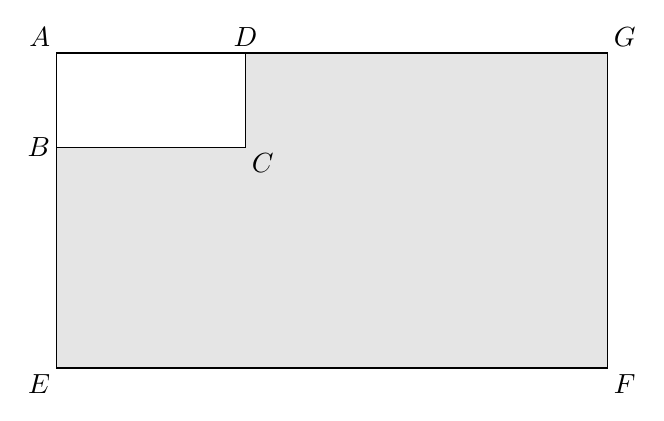
\begin{tikzpicture}[x=1cm,y=1cm,line width=.6pt,font=\normalsize]
% shaded expansion region: large AEFG minus small ABCD (even odd rule)
\fill[gray!20,even odd rule] (0,0) rectangle (7,4) (0,2.8) rectangle (2.4,4);
% outer rectangle AEFG
\draw (0,0) rectangle (7,4);
% inner cutout edges B-C-D
\draw (0,2.8) -- (2.4,2.8) -- (2.4,4);
% labels (offset 2pt, clear of lines)
\node[inner sep=0pt,anchor=south east,xshift=-2pt,yshift=2pt] at (0,4) {$A$};
\node[inner sep=0pt,anchor=east,xshift=-2pt] at (0,2.8) {$B$};
\node[inner sep=0pt,anchor=north east,xshift=-2pt,yshift=-2pt] at (0,0) {$E$};
\node[inner sep=0pt,anchor=south,yshift=2pt] at (2.4,4) {$D$};
\node[inner sep=0pt,anchor=south west,xshift=2pt,yshift=2pt] at (7,4) {$G$};
\node[inner sep=0pt,anchor=north west,xshift=2pt,yshift=-2pt] at (2.4,2.8) {$C$};
\node[inner sep=0pt,anchor=north west,xshift=2pt,yshift=-2pt] at (7,0) {$F$};
\end{tikzpicture}
